\section{Kinect Software}\label{Software}

(Essenz auf dem, was Kinect für mich erledigt theorie, mathematische Berechnung tiefe und skeletonstream usw)

Rauminformationen für Software
Vorteil: Günstig, leicht zu entwickeln, da SDK vorhanden

Da das Produkt Xbox Kinect bereits vor einigen Jahren auf den Markt kam, hatten die Entwickler Zeit, um ein SDK zu entwickeln, was alle wichtigen Programmfunktionen bereits enthält. Dies macht es einem Entwickler relativ leicht eine Anwendung zu erstellen, die bestimmte Kinect-Funktionen bereitstellt. 

\begin{description}
	\item[Die Hardware liefert folgende Werte:]~\par
	\begin{itemize}
		\item Audiosignale inkl. Richtungswert des Microphonarrays
		\item RGB Bildsignal der Kamera
		\item Tiefensignal
	\end{itemize}
\end{description}

\noindent
Für dieses Projekt sind die Audiodaten jedoch irrelevant. Wichtig sind primär die Bilddaten inklusive Tiefenwerte.
Das Kinect SDK bietet bereits standardmäßig Zugriff auf diese Werte. Dabei können im Programm bestimmte Proxyobjekte registriert und abgefragt werden. Für dieses Projekt ist das Skeletonobjekt von großer Bedeutung. Anhand von Vergleichsmustern erzeugt die Software -nicht Kinect!- einen sog. Skeletonstream, der versucht die Position eines menschlichen Skeletts im Kinect Koordinatenraum abzubilden.\cite{SWB-376536934}

\subsection{Der Skeletonstream}
Damit die Bewegungen eines Benutzers mittels Kinect erkannt und im Programm verarbeitet werden können, werden im Tiefenstream bestimmte Bereiche definiert und mit bestehenden Mustern verglichen. Somit können die einzelnen Gelenke des menschlichen Skeletts (Joints) erkannt und in Zusammenhang gebracht werden. Als Entwickler können diese dann in einem Skelettobjekt mit der erkannten Genauigkeit ausgelesen und verwendet werden. Für die Erkennung der Armbewegungen werden Schulter-, Ellenbogen-, Hand- und Hüftjoints benötigt (Siehe Realisierung).

\begin{figure}[H]						
	\centering							
	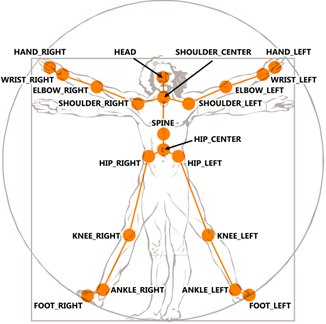
\includegraphics[scale=1.0]{Bilder/kinect_joints.png}			
	\caption{Kinect Joints \cite{ws:microsoft_jointType}}						
	\label{f:kinect_joints}						
\end{figure}



(Technischer Hintergrund der Berechnung -> Bild mit verschiedenen Farben für SKelettbereiche, aber nicht öffentlich, da Microsoft Geheimnis)

(Bild Kinect Koordinatenraum)
(Bild mehrere User im Kinectraum)

\todo{SDK Funktionen erklären: skelton, mehrere user, deep stream, color stream}
\todo{Screenshot von Deep Stream (Kinect Studio)}
\todo{Unterschied Microsoft SDK und Freie Implementierung OpenNI}
\todo{Bild von Kinect-Koordinatensystem -> Bezug auf Nao}



Dieser Stream berechnet anhand der Tiefendaten und der RGB-Daten werte für ein Menschliches Skelett:

-Armwinkel
-Positionen
-Kinectraum...


DELME\cite{hertzberg2009mobile}
